% 重排作者联系方式:econsunrq@outlook.com

% -------------------------------------------------------- 导言

\documentclass[a4paper]{article}

\usepackage[UTF8]{ctex}    % 中文
\usepackage{titlesec}      % 
\usepackage{appendix}      % 附录
\usepackage{tocloft}       % 目录
\usepackage{multicol}      % 分栏
\usepackage{geometry}      % 页面
\usepackage{fancyhdr}      % 眉脚
\usepackage{indentfirst}   % 缩进
\usepackage{graphicx}      % 图片
\usepackage{CJKfntef}      % 着重
\usepackage{pifont}        % 注音
\usepackage{enumitem}      % enumerate

% 基本设置
\geometry{left=2cm,right=2cm,top=2cm,bottom=2cm}
\setlength\parindent{2em}
\lineskip=5pt

\pagestyle{fancy}
\fancyhf{}
\fancyhead[R]{\textbf{GB/T 15834—2011}}
\fancyfoot[C]{\thepage}
\renewcommand{\headrulewidth}{0pt}
\renewcommand{\footrulewidth}{0pt}

% 设置 enumerate 环境
\setlist[enumerate,1]{label=\textbf{示例\arabic*}:,labelsep=0pt,left=1em, align=left,topsep=1pt,parsep=1pt}

% 设置计数器
\setcounter{secnumdepth}{4}
\setcounter{tocdepth}{2}
\newcounter{mycounter}[subsubsection]
\renewcommand{\themycounter}{\textbf{\thesubsubsection.\arabic{mycounter}}}
\newcounter{hercounter}[subsubsection]
\renewcommand{\thehercounter}{\textbf{\thesubsection.\arabic{hercounter}}}

% 命令
\newcommand{\zhu}{\textbf{注}:}
\renewcommand{\contentsname}{}

\begin{document}

\thispagestyle{empty}
\newgeometry{left=1cm,right=0.9cm,top=1cm,bottom=1cm}

% 顶部
\flushleft{\textbf{ICS} 01.140.10\\\textbf{A} 19}

\hfill{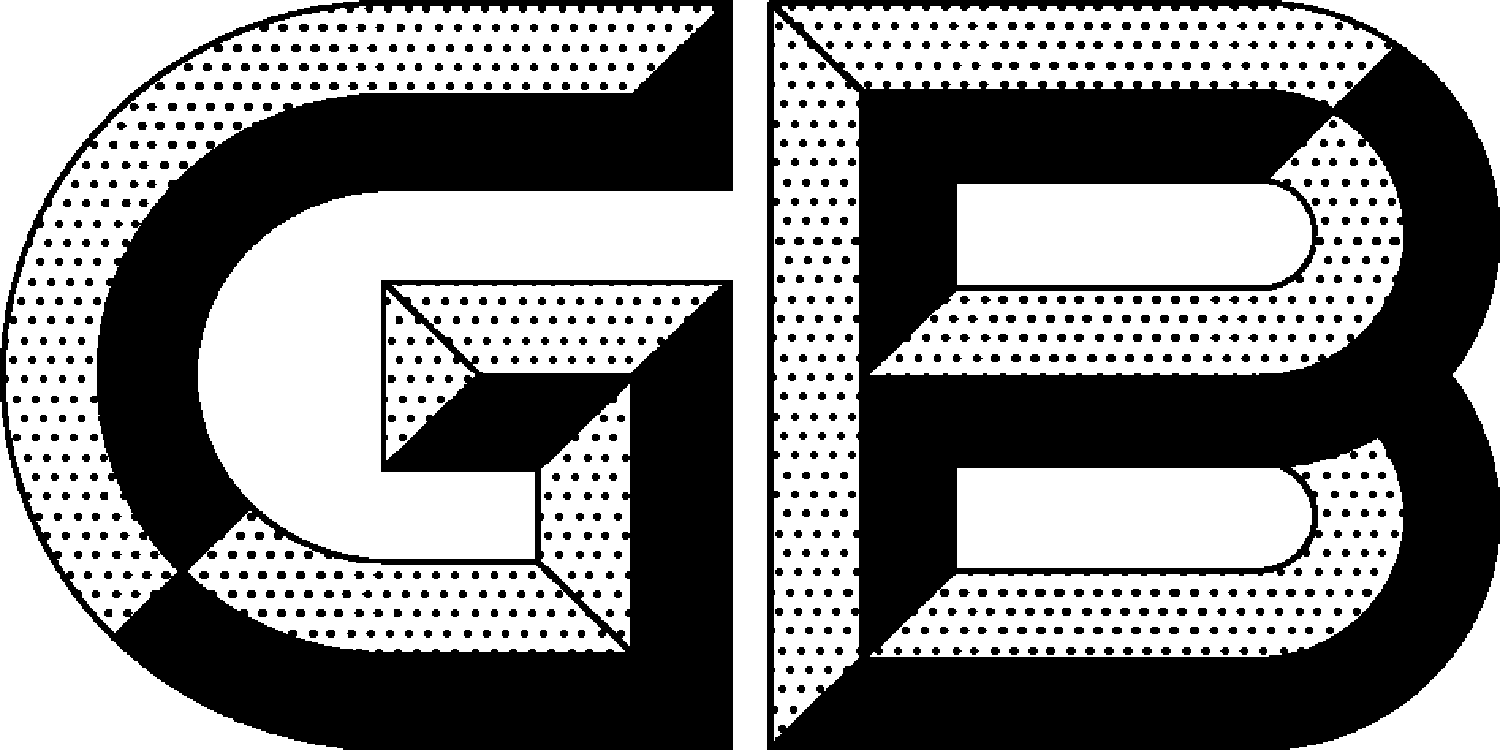
\includegraphics[width=4.5cm]{GB.png}}
\vspace{0.7cm}

{\fontsize{28pt}{0pt}{\textbf{中\hfill 华\hfill 人\hfill 民\hfill 共\hfill 和\hfill 国\hfill 国\hfill 家\hfill 标\hfill 准}}}
\vspace{0.5cm}

\hfill{\large{\textbf{GB/T 15834—2011}}}

\hfill{\small{代替 GB/T 15834—1995\,}}

\vspace{1mm}

\rule{\textwidth}{0.3mm}

\vspace{4cm}

% 中部
\begin{center}
    {\fontsize{28pt}{0pt}{\textbf{标\hspace{0.5em}点\hspace{0.5em}符\hspace{0.5em}号\hspace{0.5em}用\hspace{0.5em}法}}}
    \vspace{0.5cm}

    \Large{\textbf{General rules for punctuation}}
\end{center}

\vspace{11cm}

% 底部
\rule{\textwidth}{0.3mm}

\vspace{0.2cm}

\textbf{\large 2011-12-30 发布 \hfill 2012-06-01 实施}

% -------------------------------------------------------- 目录

\newpage
\restoregeometry
\thispagestyle{empty}

\begin{center}
    \Large{\textbf{目\hspace{2em}次}}
\end{center}
\vspace{0.5cm}

\begin{multicols}{2}
    \tableofcontents
\end{multicols}

\thispagestyle{empty}

% -------------------------------------------------------- 前页

\newpage

\pagenumbering{Roman}

\begin{center}
    \Large{\textbf{前\hspace{2em}言}}
\end{center}
\vspace{0.5cm}

{本标准按照 GB/T 1.1—2009 给出的规则起草。}

{本标准替代 GB/T 15834—1995,与 GB/T 15834—1995 相比,主要变化如下:}

\begin{enumerate}[label=——,labelsep=0pt,left=0em, align=left,topsep=1pt,parsep=1pt]
    \item 根据我国国家标准编写规则(GB/T 1.1—2009),对本标准的编排和表述做了全面修改;
    \item 更换了大部分示例,使之更简短、通俗、规范;
    \item 增加了对术语“标点符号”和“语段”的定义(2.1 / 2.5);
    \item 对术语“复句”和“分句”的定义做了修改(2.3 / 2.4);
    \item 对句末点号(句号、问号、叹号)的定义做了修改,更强调句末点号与句子语气之间的关系(4.1.1 / 4.2.1 / 4.3.1);
    \item 对逗号的基本用法作了补充(4.4.3);
    \item 增加了不同形式括号用法的示例(4.9.3);
    \item 省略号的形式统一为六连点“……”,但在特定情况下允许连用(4.11);
    \item 取消了连接号中原有的二字线。将连接号形式规范为短横线“\,-\,”、一字线“\,—\,”和波纹线“\,~\,”,并对三者的功能做了归并与划分(4.13);
    \item 明确了书名号的使用范围(4.15 / A.13);
    \item 增加了分隔号的用法说明(4.17);
    \item \;“标点符号的位置”一章的标题改为“标点符号的位置和书写形式”,并增加了使用中文输入软件处理标点符号时的相关规范(第 5 章);
    \item 增加了“附录”:附录 A 为规范性附录,主要说明标点符号不能怎样使用和对标点符号用法加以补充说明,以解决目前使用混乱或争议较大的问题。附录 B 为资料性附录,对功能有交叉的标点符号的用法做了区分,并对标点符号误用高发环境下的规范用法做了说明。
\end{enumerate}

{本标准由教育部语言文字信息管理司提出并归口。}

{本标准主要起草单位:北京大学。}

{本标准主要起草人:沈阳、刘妍、于泳波、翁珊珊。}

{本标准所替代标准的历次版本发布情况为:}

\begin{enumerate}[label=——,labelsep=0pt,left=0em, align=left,topsep=1pt,parsep=1pt]
    \item GB/T 15834—1995。
\end{enumerate}

% -------------------------------------------------------- 正文

\newpage

\pagenumbering{arabic}

\begin{center}
    \Large{\textbf{标\hspace{0.5em}点\hspace{0.5em}符\hspace{0.5em}号\hspace{0.5em}用\hspace{0.5em}法}}
\end{center}
\vspace{0.5cm}

\section{范围}

本标准规定了现代汉语标点符号的用法。

本标准适用于汉语的书面语(包括汉语和外语混合排版时的汉语部分)

\section{术语和定义}

下列术语和定义适用于本文件。

\subsection{标点符号 punctuation}

辅助文字记录语言的符号,是书面语的有机组成部分,用来表示语句的停顿、语气以及标示某些成分(主要是词语)的特性性质和作用。

\textbf{注}:
数字符号、货币符号、校勘符号、辞书符号、注音符号等特殊领域的专门符号不属于标点符号。

\subsection{句子 sentence}

前后都有较大的停顿、带有一定的语气和语调、表达相对完整意义的语言单位。

\subsection{复句 complex sentence}

由两个或多个在意义上有密切关系的分句组成的语言单位,包括简单复句(内部只有一层语义关系)和多重复句(内部包含多层语义关系)。

\subsection{分句 clause}

复句内两个或多个前后有停顿、表达相对完整意义、不带有句末语气和语调、有的前面可添加关联词语的语言单位。

\subsection{语段 expression}

指语言片段,是对各种语言单位(如词、短语、句子、复句等)不做特别区分时的统称。

\section{标点符号的种类}

\subsection{点号}

点号的作用是点断,主要表示停顿和语气。分别为句末点号和句内点号。

\subsubsection{句末点号}

用于句末的点号,表示句末停顿和句子的语气。包括句号、问号、叹号。

\subsubsection{句内点号}

用于句内的点号,表示句内各种不同性质的停顿。包括逗号、顿号、分号、冒号。

\subsection{标号}

标号的作用是标明,主要标示某些成分(主要是词语)的特定性质和作用。包括引号、括号、破折号、省略号、着重号、连接号、间隔号、书名号、专名号、分隔号。

\section{标点符号的定义、形式和用法}

\subsection{句号}

\subsubsection{定义}

句末点号的一种,主要表示句子的陈述语气。

\subsubsection{形式}

句号的形式是“\,。”。

\subsubsection{基本用法}
\vspace{1em}

\refstepcounter{mycounter}\themycounter\hspace{1em}
用于句子末尾,表示陈述语气。使用句号主要根据语段前后有较大停顿、带有陈述语气和语调,并不取决于句子的长短。

\begin{enumerate}
    \item 北京是中华人民共和国的首都。
    \item (甲:咱们走着去吧?)乙:好。
\end{enumerate}
\vspace{1em}

\refstepcounter{mycounter}\themycounter\hspace{1em}
有时也可表示较缓和的祈使语气和感叹语气。

\begin{enumerate}
    \item 请您稍等一下。
    \item 我不由地感到,这些普通劳动者也同样是很值得尊敬的。
\end{enumerate}

\subsection{问号}

\subsubsection{定义}

句末点号的一种,主要表示句子的疑问语气。

\subsubsection{形式}

问号的形式是“\,?”。

\subsubsection{基本用法}
\vspace{1em}

\refstepcounter{mycounter}\themycounter\hspace{1em}
用于句子末尾,表示疑问语气(包括反问、设问等疑问类型)。使用问号主要根据语段前后有较大停顿、带有疑问语气和语调,并不取决于句子的长短。

\begin{enumerate}
    \item 你怎么还不回家去呢?
    \item 难道这些普通战士不值得歌颂吗?
    \item (一个外国人,不远万里来到中国,帮助中国的抗日战争。)这是什么精神?这是国际主义的精神。
\end{enumerate}
\vspace{1em}

\refstepcounter{mycounter}\themycounter\hspace{1em}
选择问句中,通常只在最后一个选项的末尾用问号,各个选项之间一般用逗号隔开。当选项较短且选项之间几乎没有停顿时,选项之间可不用逗号。当选项较多或较长,或有意突出每个选项的独立性时,也可每个选项之后都用问号。

\begin{enumerate}
    \item 诗中记述的这场战争究竟是真实的历史描述,还是诗人的虚构?
    \item 这是巧合还是有意安排?
    \item 要一个什么样的结尾:现实主义的?传统的?大团圆的?荒诞的?民族形式的?有象征意义的?
    \item (他看着我的作品称赞了我。)但到底是称赞我什么:是有几处画得好?还是什么都敢画?抑或只是一种对于失败者的无可奈何的安慰?我不得而知。
    \item 这一切都是由客观的条件造成的?还是由行为的惯性造成的?
\end{enumerate}
\vspace{1em}

\refstepcounter{mycounter}\themycounter\hspace{1em}
在多个问句连用或表达疑问语气加重时,可叠用问号。通常应先单用,再叠用,最多叠用三个问号。在没有异常强烈的情感表达需要时不宜叠用问号。

\begin{enumerate}[label=\textbf{示例:}]
    \item 这就是你的做法吗?你这个总经理是怎么当的??你怎么竟敢这样欺骗消费者???
\end{enumerate}
\vspace{1em}

\refstepcounter{mycounter}\themycounter\hspace{1em}
问号也有标号的用法,即用于句内,表示存疑或不详。

\begin{enumerate}
    \item 马致远(1250?-1321),大都人,元代戏曲家、散曲家。
    \item 钟嵘(?-518),颍川长社人,南朝梁代文学批评家。
    \item 出现这样的文字错误,说明作者(编者?校者?)很不认真。
\end{enumerate}

\subsection{叹号}

\subsubsection{定义}

句末点号的一种,主要表示句子的感叹语气。

\subsubsection{形式}

叹号的形式是“\,!”。

\subsubsection{基本用法}
\vspace{1em}

\refstepcounter{mycounter}\themycounter\hspace{1em}
用于句子末尾,表示感叹语气,有时也可表示强烈的祈使语气、反问语气等。使用叹号主要根据语段前后有较大停顿、带有感叹语气和语调或带有强烈的祈使语气、反问语气和语调,并不取决于句子的长短。

\begin{enumerate}
    \item 才一年不见,这孩子都长这么高啦!
    \item 你给我住嘴!
    \item 谁知道他今天是怎么搞的!
\end{enumerate}
\vspace{1em}

\refstepcounter{mycounter}\themycounter\hspace{1em}
用于拟声词后,表示声援短促或突然。

\begin{enumerate}
    \item 咔嚓!一道闪电划破了夜空。
    \item 咚!咚咚!突然传来一阵急促的敲门声。
\end{enumerate}
\vspace{1em}

\refstepcounter{mycounter}\themycounter\hspace{1em}
表示声音巨大或声音不断加大时,可叠用叹号;表达强烈语气时,也可叠用叹号,最多叠用三个叹号。在没有异常强烈的情感表达需要时不宜叠用叹号。

\begin{enumerate}
    \item 轰!!在这天崩地塌的声音中,女娲猛然醒来。
    \item 我要揭露!我要控诉!!我要以死抗争!!!
\end{enumerate}
\vspace{1em}

\refstepcounter{mycounter}\themycounter\hspace{1em}
当句子包含疑问、感叹两种语气且都比较强烈时(如带有强烈情感的反问句和带有惊愕语气的疑问句),可在问号后再加叹号(问号、叹号各一)。

\begin{enumerate}
    \item 这么点困难就能把我们吓倒吗?!
    \item 他连这些最起码的常识都不懂,还敢说自己是高科技人材?!
\end{enumerate}

\subsection{逗号}

\subsubsection{定义}

句内点号的一种,主要表示句子或语段内部的一般性停顿。

\subsubsection{形式}

逗号的形式是“\,,”。

\subsubsection{基本用法}
\vspace{1em}

\refstepcounter{mycounter}\themycounter\hspace{1em}
复句内各分句之间的停顿,除了有时用分号(见 4.6.3.1),一般都用逗号。

\begin{enumerate}
    \item 不是人们的意识决定了人们的存在,而是人们的社会存在决定人们的意识。
    \item 学历史使人更明智,学文学使人更聪慧,学数学使人更精细,学考古使人更深沉。
    \item 要是不相信我们的理论能反映现实,要是不相信我们的世界有内在和谐,那就不可能有科学。
\end{enumerate}
\vspace{1em}

\refstepcounter{mycounter}\themycounter\hspace{1em}
用于下列各种语法位置:

a)
较长的主语之后。

\hspace{1em}\textbf{示例 1}:
苏州园林建筑各种门窗的精美设计和雕镂功夫,都令人叹为观止。

b)
句首的状语之后。

\hspace{1em}\textbf{示例 2}:
在苍茫的大海上,狂风卷集着乌云。

c)
较长的宾语之前。

\hspace{1em}\textbf{示例 3}:
有的考古工作者认为,南方古猿生存于上新世至更新世的初级和中期。

d)
带句内语气词的主语(或其他部分)之后,或带句内语气词的并列成分之间。

\hspace{1em}\textbf{示例 4}:
他呢,倒是很乐意地、全神贯注地干起来了。

\hspace{1em}\textbf{示例 5}:
(那是个没有月亮的夜晚)可是整个村子——白房顶啦,白树木啦,雪堆啦,全看得见。

e)
较长的主语中间、谓语中间或宾语中间。

\hspace{1em}\textbf{示例 6}:
母亲沉痛的诉说,以及亲眼见到的事实,都启发了我幼年时期追求真理的思想。

\hspace{1em}\textbf{示例 7}:
那姑娘头戴一顶草帽,身穿一条绿色裙子,腰间还系着一根橙色的腰带。

\hspace{1em}\textbf{示例 8}:
必须懂得,对于文化传统,既不能不分青红皂白统统抛弃,也不能不管精华糟粕全盘继承。

f)
前置的谓语之后或后置的状语、定语之前。

\hspace{1em}\textbf{示例 9}:
真美啊,这条蜿蜒的林间小路。

\hspace{1em}\textbf{示例 10}:
她吃力地站了起来,慢慢地。

\hspace{1em}\textbf{示例 11}:
我只是一个人,孤孤单单的。
\vspace{1em}

\refstepcounter{mycounter}\themycounter\hspace{1em}
用于下列各种停顿处。

a)
复指成分或插说成分前后。

\hspace{1em}\textbf{示例 1}:
老张,就是原来的办公室主任,上星期已经调走了。

\hspace{1em}\textbf{示例 2}:
车,不用说,当然是头等。

b)
语气缓和的感叹语、称谓语或呼唤语之后。

\hspace{1em}\textbf{示例 3}:
哎哟,这儿,快给我揉揉。

\hspace{1em}\textbf{示例 4}:
大娘,您到哪儿去啊?

\hspace{1em}\textbf{示例 5}:
喂,你是哪个单位的?

c)
某些序次语(“第”字头,“其”字头及“首先”类序次语)之后。

\hspace{1em}\textbf{示例 6}:
为什么许多人都有长不大的感觉呢?原因有三:第一,父母总认为自己比孩子成熟;第二,父母总要以自己的标准来衡量孩子;第三,父母出于爱心而总不想让孩子在成长的过程中走弯路。

\hspace{1em}\textbf{示例 7}:
《玄秘塔碑》所以成为书法的范本,不外乎以下几方面的因素:其一,具有楷书点画、构体的典范性;其二,承上启下,成为唐楷的极致;其三,字如其人,爱人及字,柳公权高尚的书品、人品为后人所崇仰。

\hspace{1em}\textbf{示例 8}:
下面从三个方面讲讲语言的污染问题:首先,是特殊语言环境中的语言污染问题;其次,是滥用缩略语引起的语言污染问题;再次,是空话和废话引起的语言污染问题。

\subsection{顿号}

\subsubsection{定义}

句內点号的一种,表示语段中并列词语之间或某些序次语之后的停顿。

\subsubsection{形式}

顿号的形式是“、”。

\subsubsection{基本用法}
\vspace{1em}

\refstepcounter{mycounter}\themycounter\hspace{1em}
用于并列词语之间。

\begin{enumerate}
    \item 这里有自由、民主、平等、开放的风气和氛围。
    \item 造型科学、技艺精湛、气韵生动,是盛唐石雕的特色。
\end{enumerate}
\vspace{1em}

\refstepcounter{mycounter}\themycounter\hspace{1em}
用于需要停顿的重复词语之间。

\begin{enumerate}[label=\textbf{示例:},labelsep=0pt,left=2em, align=left,topsep=1pt,parsep=1pt]
    \item 他几次三番、几次三番地辩解着。
\end{enumerate}
\vspace{1em}

\refstepcounter{mycounter}\themycounter\hspace{1em}
用于某些序次语(不带括号的汉字数字或“天干地支”类序次语)之后。

\begin{enumerate}
    \item 我准备讲两个问题:一、逻辑学是什么?二、怎样学好逻辑学?
    \item 风格的具体内容主要有以下四点:甲、题材;乙、用字;丙、表达;丁、色彩。
\end{enumerate}
\vspace{1em}

\refstepcounter{mycounter}\themycounter\hspace{1em}
相邻或相近两数字连用表示概数通常不用顿号。若相邻两数字连用为缩略形式,宜用顿号。

\begin{enumerate}
    \item 飞机在 6\,000 米高空水平飞行时,只能看到两侧八九公里和前方一二十公里范围内的地面。
    \item 这种凶猛的动物常常三五成群地外出觅食和活动。
    \item 农业是国民经济的基础,也是二、三产业的基础。
\end{enumerate}
\vspace{1em}

\refstepcounter{mycounter}\themycounter\hspace{1em}
标有引号的并列成分之间、标有书名号的并列成分之间通常不用顿号。若有其他成分插在并列的引号之间或并列的书名号之间(如引语或书名号之后还有括注),宜用顿号。

\begin{enumerate}
    \item “日”“月”构成“明”字。
    \item 店里挂着“顾客就是上帝”“质量就是生命”等横幅。
    \item 《红楼梦》《三国演义》《西游记》《水浒传》,是我国长篇小说的四大名著。
    \item 李白的“白发三千丈”(《秋浦歌》)、“朝如青丝暮成雪”(《将进酒》)都是脍炙人口的诗句。
    \item 办公室里订有《人民日报》(海外版)、《光明日报》和《时代周刊》等报刊。
\end{enumerate}

\subsection{分号}

\subsubsection{定义}

句內点号的一种,表示复句内部并列关系分句之间的停顿,以及非并列关系的多重复句中第一层分局之间的停顿。

\subsubsection{形式}

分号的形式是“;”。

\subsubsection{基本用法}
\vspace{1em}

\refstepcounter{mycounter}\themycounter\hspace{1em}
表示复句内部并列关系的分句(尤其当分句内部还有逗号时)之间的停顿。

\begin{enumerate}
    \item 语言文字的学习,就理解方面说,就是得到一种知识;就运用方面说,是养成一种习惯。
    \item 内容有分量,尽管文章短小,也是有分量的;内容没有分量,即使写得再长也没有用。
\end{enumerate}
\vspace{1em}

\refstepcounter{mycounter}\themycounter\hspace{1em}
表示非并列关系的多重复句中第一层分句(主要是选择、转折等关系)之间的停顿。

\begin{enumerate}
    \item 人还没看见,已经先听见歌声了;或者人已经转过山头望不见了,歌声还余音袅袅。
    \item 尽管人民革命的力量在开始时总是弱小的,所以总是受压迫;但是由于革命的力量代表历史发展的方向,因此本质上又是不可战胜的。
    \item 不管一个人如何伟大,也总是生活在一定的环境和条件下;因此,个人的见解总难免带有某种局限性。
    \item 昨天夜里下了一场雨,以为可以凉快些;谁知没有凉快下来,反而更热了。
\end{enumerate}
\vspace{1em}

\refstepcounter{mycounter}\themycounter\hspace{1em}
用于分项列举的各项之间。

\begin{enumerate}[label=\textbf{示例:},labelsep=0pt,left=2em, align=left,topsep=1pt,parsep=1pt]
    \item 特聘教授的岗位职责为:一、讲授本学科的主干基础课程;二、主持本学科的重大科研项目;三、领导本学科的学术队伍建设;四、带领本学科赶超或保持世界先进水平。
\end{enumerate}


\subsection{冒号}

\subsubsection{定义}

句内点号的一种,表示语段中提示下文或总结上文的停顿。

\subsubsection{形式}

冒号的形式是“\,:”。

\subsubsection{基本用法}
\vspace{1em}

\refstepcounter{mycounter}\themycounter\hspace{1em}
用于总说性或提示性词语(如“说”“例如”“证明”等)之后,表示提示下文。

\begin{enumerate}
    \item 北京紫禁城有四座城门:午门、神武门、东华门和西华门。
    \item 她高兴的说:“咱们去好好庆祝一下吧!”
    \item 小王笑着点了点头:“我就是这么想的。”
    \item 这一事实证明:人能创造环境,环境同样也能创造人。
\end{enumerate}
\vspace{1em}

\refstepcounter{mycounter}\themycounter\hspace{1em}
表示总结上文。

\begin{enumerate}[label=\textbf{示例:},labelsep=0pt,left=2em, align=left,topsep=1pt,parsep=1pt]
    \item 张华上了大学,李萍进了技校,我当了工人:我们都有美好的前途。
\end{enumerate}
\vspace{1em}

\refstepcounter{mycounter}\themycounter\hspace{1em}
用在需要说明的词语之后,表示注释和说明。

\begin{enumerate}
    \item (本市将举办首届大型书市。)主办单位:市文化局;承办单位:市图书进口公司;时间:8 月 15 日—— 20 日;地点:市体育馆观众休息厅。
    \item (做阅读理解题有两个办法。)办法之一:先读题干,再读原文,带着问题有针对性地读课文。办法之二:直接读原文,读完再做题,减少先入为主的干扰。
\end{enumerate}
\vspace{1em}

\refstepcounter{mycounter}\themycounter\hspace{1em}
用于书信、讲话稿中称谓语或称呼语之后。

\begin{enumerate}
    \item 广平先生:……
    \item 同志们、朋友们:……
\end{enumerate}
\vspace{1em}

\refstepcounter{mycounter}\themycounter\hspace{1em}
一个句子内部一般不用套用冒号。在列举式或条文式表述中,如不得不套用冒号时,宜另起段落来显示各个层次。

\begin{enumerate}[label=\textbf{示例:},labelsep=0pt,left=2em, align=left,topsep=1pt,parsep=1pt]
    \item 第十条\quad 遗嘱按照下列顺序继承:\\第一顺序:配偶、子女、父母。\\第二顺序:兄弟姐妹、祖父母、外祖父母。
\end{enumerate}

\subsection{引号}

\subsubsection{定义}

标号的一种,标示语段中直接引用的内容或需要特别之处的成分。

\subsubsection{形式}

引号的形式有双引号““”“””和单引号“‘’”两种。左侧的为前引号,右侧的为后引号。

\subsubsection{基本用法}
\vspace{1em}

\refstepcounter{mycounter}\themycounter\hspace{1em}
标示语段中直接引用的内容。

\begin{enumerate}[label=\textbf{示例:},labelsep=0pt,left=2em, align=left,topsep=1pt,parsep=1pt]
    \item 李白诗中就有“白发三千丈”这样极尽夸张的语句。
\end{enumerate}
\vspace{1em}

\refstepcounter{mycounter}\themycounter\hspace{1em}
标示需要着重论述或强调的内容。

\begin{enumerate}[label=\textbf{示例:},labelsep=0pt,left=2em, align=left,topsep=1pt,parsep=1pt]
    \item 这里所谓的“文”,并不是指文字,而是指文采。
\end{enumerate}
\vspace{1em}

\refstepcounter{mycounter}\themycounter\hspace{1em}
标示语段中具有特殊含义而需要特别指出的成分,如别称、简称、反语等。

\begin{enumerate}
    \item 电视被称作“第九艺术”。
    \item 人类学上常把古人化石统称为尼安德特人,简称“尼人”。
    \item 有几个“慈祥”的老板把捡来的菜叶用盐浸浸就算作工友的菜肴。
\end{enumerate}
\vspace{1em}

\refstepcounter{mycounter}\themycounter\hspace{1em}
当引号中还需要使用引号时,外面一层用双引号,里面一层用单引号。

\begin{enumerate}[label=\textbf{示例:},labelsep=0pt,left=2em, align=left,topsep=1pt,parsep=1pt]
    \item 他问:“老师,‘七月流火’是什么意思?”
\end{enumerate}
\vspace{1em}

\refstepcounter{mycounter}\themycounter\hspace{1em}
独立成段的引文如果只有一段,段首和段尾都不用引号;不止一段时,每段开头仅用前引号,只在最后一段末尾用后引号。

\begin{enumerate}[label=\textbf{示例:},labelsep=0pt,left=2em, align=left,topsep=1pt,parsep=1pt]
    \item 我曾在报纸上看到有人这样谈幸福:\\“幸福是知道自己喜欢什么和不喜欢什么。……\\“幸福是知道自己擅长什么和不擅长什么。……\\“幸福是在正确的时间做了正确的选择。……”
\end{enumerate}
\vspace{1em}

\refstepcounter{mycounter}\themycounter\hspace{1em}
在书写带月、日的事件、节日或其他特定意义的短语(含简称)时,通常只标引其中的月和日;需要突出和强调该事件或节日本身时,也可连同事件或节日一起标引。

\begin{enumerate}
    \item “5\,$\cdot$\,12”汶川大地震。
    \item “五四”以来的话剧,是我国戏剧中的新形式。
    \item 纪念“五四运动”90 周年。
\end{enumerate}

\subsection{括号}

\subsubsection{定义}

标号的一种,标示语段中的注释内容、补充说明或其他特定意义的语句。

\subsubsection{形式}

括号的主要形式是圆括号“()”,其他形式还有方括号“[ ]”、六角括号“〔〕”和方头括号“【】”等。

\subsubsection{基本用法}
\vspace{1em}

\refstepcounter{mycounter}\themycounter\hspace{1em}
标识下列各种情况,均用圆括号:

a)
标识注释内容或补充说明。

\hspace{1em}\textbf{示例 1}:
我校拥有特级教师(含已退休的)17 人。

\hspace{1em}\textbf{示例 2}:
我们不但善于破坏一个旧世界,我们还将善于建设一个新世界!(热烈鼓掌)

b)
标示订正或补加的文字。

\hspace{1em}\textbf{示例 3}:
信纸上用稚嫩的字体写着:“阿夷(姨),你好!”。

\hspace{1em}\textbf{示例 4}:
该建筑公司负责的建设工程全部达到优良工程(的标准)。

c)
标示序次语。

\hspace{1em}\textbf{示例 5}:
语言有三个要素:(1)声音;(2)结构;(3)意义。

\hspace{1em}\textbf{示例 6}:
思想有三个条件:(一)事理;(二)心理;(三)伦理。

d)
标示引语的出处。

\hspace{1em}\textbf{示例 7}:
他说得好:“未画之前,不立一格;既画之后,不留一格。”(《板桥集\,$\cdot$\,题画》)

e)标示汉语拼音注音。

\hspace{1em}\textbf{示例 8}:
“的(de)”这个字在现代汉语中最常用。
\vspace{1em}

\refstepcounter{mycounter}\themycounter\hspace{1em}
标示国籍或所属朝代时,可用方括号或六角括号。

\hspace{1em}\textbf{示例 1}:
[英] 赫胥黎《进化论与伦理学》。

\hspace{1em}\textbf{示例 2}:
〔唐〕杜甫著。
\vspace{1em}

\refstepcounter{mycounter}\themycounter\hspace{1em}
报刊标示电讯、报道的开头,可用方头括号。

\begin{enumerate}[label=\textbf{示例:},labelsep=0pt,left=2em, align=left,topsep=1pt,parsep=1pt]
    \item 【新华社南京消息】
\end{enumerate}
\vspace{1em}

\refstepcounter{mycounter}\themycounter\hspace{1em}
标示公文发文字号中的发文年份时,可用六角括号。

\begin{enumerate}[label=\textbf{示例:},labelsep=0pt,left=2em, align=left,topsep=1pt,parsep=1pt]
    \item 国发〔2011〕3 号文件
\end{enumerate}
\vspace{1em}

\refstepcounter{mycounter}\themycounter\hspace{1em}
标示被注释的词语时,可用六角括号或方头括号。

\begin{enumerate}
    \item 〔奇观〕奇伟的景象。
    \item 【爱因斯坦】物理学家。出生于德国,1933 年因受纳粹政权迫害,移居美国。
\end{enumerate}
\vspace{1em}

\refstepcounter{mycounter}\themycounter\hspace{1em}
除科技书刊中的数学、逻辑公式外,所有括号(特别是同一形式的括号)应尽量避免套用。必须套用括号时,宜采用不同的括号形式配合使用。

\begin{enumerate}[label=\textbf{示例:},labelsep=0pt,left=2em, align=left,topsep=1pt,parsep=1pt]
    \item 〔茸(róng)毛〕很细很细的毛。
\end{enumerate}

\subsection{破折号}

\subsubsection{定义}

标号的一种,标示语段中某些成分的注释、补充说明或语音、意义的变化。

\subsubsection{形式}

破折号的形式是“——”。

\subsubsection{基本用法}
\vspace{1em}

\refstepcounter{mycounter}\themycounter\hspace{1em}
标示注释内容或补充说明(也可用括号,见 4.9.3.1;二者的区别另见 B.1.7)。

\begin{enumerate}
    \item 一个矮小而结实的日本中年人——内山老板走了过来。
    \item 我一直坚持读书,想借此唤起弟妹对生活的希望——无论环境多么困难。
\end{enumerate}
\vspace{1em}

\refstepcounter{mycounter}\themycounter\hspace{1em}
标示插入语(也可用逗号,见 4.4.3.3)。

\begin{enumerate}[label=\textbf{示例:},labelsep=0pt,left=2em, align=left,topsep=1pt,parsep=1pt]
    \item 这简直就是——说得不客气点——无耻的勾当!
\end{enumerate}
\vspace{1em}

\refstepcounter{mycounter}\themycounter\hspace{1em}
标示总结上文或提示下文(也可用冒号,见 4.7.3.1、4.7.3.2)。

\begin{enumerate}
    \item 坚强,纯洁,严于律己,客观公正——这一切都难得地集中体现在一个人身上。
    \item 画家开始娓娓道来——\\数年前的一个寒冬,……
\end{enumerate}
\vspace{1em}

\refstepcounter{mycounter}\themycounter\hspace{1em}
标示话题的转换。

\begin{enumerate}[label=\textbf{示例:},labelsep=0pt,left=2em, align=left,topsep=1pt,parsep=1pt]
    \item “好香的干菜,——听到风声了吗?”赵七爷低声说道。
\end{enumerate}
\vspace{1em}

\refstepcounter{mycounter}\themycounter\hspace{1em}
标示声音的延长。

\begin{enumerate}[label=\textbf{示例:},labelsep=0pt,left=2em, align=left,topsep=1pt,parsep=1pt]
    \item “嘎——”传来一声水禽被惊动的鸣叫。
\end{enumerate}
\vspace{1em}

\refstepcounter{mycounter}\themycounter\hspace{1em}标示话语的中断或间隔。

\begin{enumerate}
    \item “班长他牺——”小马话没说完就大哭起来。
    \item “亲爱的妈妈,你不知道我多爱您。——还有你,我的孩子!”
\end{enumerate}
\vspace{1em}

\refstepcounter{mycounter}\themycounter\hspace{1em}
标示引出对话。

\begin{enumerate}[label=\textbf{示例:},labelsep=0pt,left=2em, align=left,topsep=1pt,parsep=1pt]
    \item ——你长大后想成为科学家吗?\\——当然想了!
\end{enumerate}
\vspace{1em}

\refstepcounter{mycounter}\themycounter\hspace{1em}
标示事项列举分承。

\begin{enumerate}[label=\textbf{示例:},labelsep=0pt,left=2em, align=left,topsep=1pt,parsep=1pt]
    \item 根据研究对象的不同,环境物理学分为以下五个分支学科:\\环境声学;\\环境光学;\\环境热学;\\环境电磁学;\\环境空气动力学。
\end{enumerate}
\vspace{1em}

\refstepcounter{mycounter}\themycounter\hspace{1em}
用于副标题之前。

\begin{enumerate}[label=\textbf{示例:},labelsep=0pt,left=2em, align=left,topsep=1pt,parsep=1pt]
    \item 飞向太平洋\\我国新型号运载火箭发射目击记
\end{enumerate}
\vspace{1em}

\refstepcounter{mycounter}\themycounter\hspace{1em}
用于引文、注文后,标示作者、出处或注释者。

\begin{enumerate}
    \item 先天下之忧而忧,后天下之乐而乐。\\\hspace{12em}——《孟子》
    \item 乐浪海中有倭人,分为百余国。\\\hspace{12em}——《汉书》
    \item 很多人写好信后把信笺折成方胜形,我看大可不必。(方胜,指古代妇女戴的方形首饰,用彩绸等制作,由两个斜方部位叠合而成。——编者注)
\end{enumerate}

\subsection{省略号}

\subsubsection{定义}

标号的一种,标示语段中某些内容的省略及意义的断续等。

\subsubsection{形式}

省略号的形式是“……”。

\subsubsection{基本用法}
\vspace{1em}

\refstepcounter{mycounter}\themycounter\hspace{1em}
标示引文的省略。

\begin{enumerate}[label=\textbf{示例:},labelsep=0pt,left=2em, align=left,topsep=1pt,parsep=1pt]
    \item 我们齐声朗诵起来:“……俱往矣,数风流人物,还看今朝。”
\end{enumerate}
\vspace{1em}

\refstepcounter{mycounter}\themycounter\hspace{1em}
标示列举或重复词语的省略。

\begin{enumerate}
    \item 对政治的敏感,对生活的敏感,对性格的敏感,……这都是作家必须要有的素质。
    \item 他气得连声说:“好,好……算我没说。”
\end{enumerate}
\vspace{1em}

\refstepcounter{mycounter}\themycounter\hspace{1em}
标示语义未尽。

\begin{enumerate}
    \item 在人迹罕至的深山密林里,假如突然看见一缕炊烟,……
    \item 你这样干,未免太……!
\end{enumerate}
\vspace{1em}

\refstepcounter{mycounter}\themycounter\hspace{1em}
标示说话时断断续续.

\begin{enumerate}[label=\textbf{示例:},labelsep=0pt,left=2em, align=left,topsep=1pt,parsep=1pt]
    \item 她磕磕巴巴地说:“可是……太太……我不知道……你一定是认错人了。”
\end{enumerate}
\vspace{1em}

\refstepcounter{mycounter}\themycounter\hspace{1em}
标示对话中的沉默不语。

\begin{enumerate}[label=\textbf{示例:},labelsep=0pt,left=2em, align=left,topsep=1pt,parsep=1pt]
    \item “还没结婚吧?”\\“……”他飞红了脸,更加忸怩起来。
\end{enumerate}
\vspace{1em}

\refstepcounter{mycounter}\themycounter\hspace{1em}
标示特定的成分缺失。

\begin{enumerate}[label=\textbf{示例:},labelsep=0pt,left=2em, align=left,topsep=1pt,parsep=1pt]
    \item 只要……就……
\end{enumerate}
\vspace{1em}

\refstepcounter{mycounter}\themycounter\hspace{1em}
在标示诗行、段落的省略时,可连用两个省略号(即相当于十二连点)。

\begin{enumerate}
    \item 从隔壁房间传来缓缓而抑扬顿挫的吟咏声——\\床前明月光,疑是地上霜。\\…………
    \item 该刊根据工作质量、上稿数量、参与程度等方面的表现,评选出了高校十佳记者站。还根据发稿数量、提供新闻线索情况以及对刊物的关注度等,评选出了十佳通讯员。\\…………
\end{enumerate}

\subsection{着重号}

\subsubsection{定义}

标号的一种,标示语段中某些重要的或需要指明的文字。

\subsubsection{形式}

着重号的形式是“.”标注在相应文字的下方。

\subsubsection{基本用法}
\vspace{1em}

\refstepcounter{mycounter}\themycounter\hspace{1em}
标示语段中重要的文字。

\begin{enumerate}
    \item 诗人需要\CJKunderdot{表现},而不是\CJKunderdot{证明}。
    \item 下面对本文的理解,\CJKunderdot{不正确}的一项是:……
\end{enumerate}
\vspace{1em}

\refstepcounter{mycounter}\themycounter\hspace{1em}
标示语段中需要指明的文字。

\begin{enumerate}[label=\textbf{示例:},labelsep=0pt,left=2em, align=left,topsep=1pt,parsep=1pt]
    \item 下边加点的字,除了在词中的读法外,还有哪些读法?\\\CJKunderdot{着}急\quad 子\CJKunderdot{弹}\quad 强\CJKunderdot{调}
\end{enumerate}

\subsection{连接号}

\subsubsection{定义}

标号的一种,标示某些相关联成分之间的连接。

\subsubsection{形式}

连接号的形式有短横线“\,-\,”、一字线“\,—\,”和波纹线“\,~\,”三种。

\subsubsection{基本用法}
\vspace{1em}

\refstepcounter{mycounter}\themycounter\hspace{1em}
标示下列各种情况,均用短横线:

a)
化合物的名称或表格、插图的编号。

\hspace{1em}\textbf{示例 1}:
3-戊酮为无色液体,对眼及皮肤有强烈刺激性。

\hspace{1em}\textbf{示例 2}:
参见下页表 2-8、表 2-9。

b)
连接号码,包括门牌号码、电话号码,以及用阿拉伯数字表示年月日等。

\hspace{1em}\textbf{示例 3}:
安宁里东路 26 号院 3-2-11 室

\hspace{1em}\textbf{示例 4}:
联系电话:010-88842603

\hspace{1em}\textbf{示例 5}:
2011-02-15

c)
在复合名词中起连接作用。

\hspace{1em}\textbf{示例 6}:
吐鲁番-哈密盆地

d)
某些产品的名称和型号。

\hspace{1em}\textbf{示例 7}:
WZ-10 直升机具有复杂天气和夜间作战的能力。

e)
汉语拼音、外来语内部的分合。

\hspace{1em}\textbf{示例 8}:
shuōshuō-xiàoxiào(说说笑笑)

\hspace{1em}\textbf{示例 9}:
盎格鲁-撒克逊人

\hspace{1em}\textbf{示例 10}:
让-雅克\,$\cdot$\,卢梭(“让-雅克”为双名)

\hspace{1em}\textbf{示例 11}:
皮埃尔\,$\cdot$\,孟戴斯-弗朗斯(“孟戴斯-弗朗斯”为复姓)
\vspace{1em}

\refstepcounter{mycounter}\themycounter\hspace{1em}
标示下列各种情况,一般用一字线,有时也可用波浪纹:

a)
标示相关项目(如时间、地域等)的起止。

\hspace{1em}\textbf{示例 1}:
沈括(1031—1095),宋朝人

\hspace{1em}\textbf{示例 2}:
2011 年 2 月 3 日—10 日

\hspace{1em}\textbf{示例 3}:
北京—上海特别旅客快车

b)
标示数值范围(由阿拉伯数字或汉字数字构成)的起止。

\hspace{1em}\textbf{示例 4}:
20~30 g

\hspace{1em}\textbf{示例 5}:
第五~ 八课

\subsection{间隔号}

\subsubsection{定义}

标号的一种,标示某些相关联成分之间的分界。

\subsubsection{形式}

间隔号的形式是“\,$\cdot$\,”。

\subsubsection{基本用法}
\vspace{1em}

\refstepcounter{mycounter}\themycounter\hspace{1em}
标示外国人名或少数民族人名内部的分界。

\begin{enumerate}
    \item 克里斯蒂娜\,$\cdot$\,罗塞蒂
    \item 阿依古丽\,$\cdot$\,买买提
\end{enumerate}
\vspace{1em}

\refstepcounter{mycounter}\themycounter\hspace{1em}
标示书名与篇(章、卷)名之间的分界。

\begin{enumerate}[label=\textbf{示例:},labelsep=0pt,left=2em, align=left,topsep=1pt,parsep=1pt]
    \item 《淮南子\,$\cdot$\,本经训》
\end{enumerate}
\vspace{1em}

\refstepcounter{mycounter}\themycounter\hspace{1em}
标示词牌、曲牌、诗体名等和题名之间的分界。

\begin{enumerate}
    \item 《沁园春\,$\cdot$\,雪》
    \item 《天净沙\,$\cdot$\,秋思》
    \item 《七律\,$\cdot$\,冬云》
\end{enumerate}
\vspace{1em}

\refstepcounter{mycounter}\themycounter\hspace{1em}
用在构成标题或栏目名称的并列词语之间。

\begin{enumerate}[label=\textbf{示例:},labelsep=0pt,left=2em, align=left,topsep=1pt,parsep=1pt]
    \item 《天\,$\cdot$\,地\,$\cdot$\,人》
\end{enumerate}
\vspace{1em}

\refstepcounter{mycounter}\themycounter\hspace{1em}
以月、日为标志的事件或节日,用汉字数字表示时,只在一、十一和十二月后用间隔号;当直接用阿拉伯数字表示时,月、日之间均用间隔号(半角字符)。

\begin{enumerate}
    \item “九一八”事变\quad “五四”运动
    \item “一\,$\cdot$\,二八”事变\quad “一二\,$\cdot$\,九”运动
    \item “3\,$\cdot$\,15”消费者权益日\quad “9\,$\cdot$\,11”恐怖袭击事件
\end{enumerate}

\subsection{书名号}

\subsubsection{定义}

标号的一种,标示语段中出现的各种作品的名称。

\subsubsection{形式}

书名号的形式有双书名号“《》”和单书名号“〈〉”。

\subsubsection{基本用法}
\vspace{1em}

\refstepcounter{mycounter}\themycounter\hspace{1em}
标示书名、卷名、篇名、刊物名、报纸名、文件名等。

\begin{enumerate}
    \item 《红楼梦》(书名)
    \item 《史记\,$\cdot$\,项羽本记》(卷名)
    \item 《论雷峰塔的倒掉》(篇名)
    \item 《每日关注》(刊物名)
    \item 《人民日报》(报纸名)
    \item 《全国农村工作会议纪要》(文件名)
\end{enumerate}
\vspace{1em}

\refstepcounter{mycounter}\themycounter\hspace{1em}
标示电影、电视、音乐、诗歌、雕塑等各类用文字、声音、图像等表现的作品的名称。

\begin{enumerate}
    \item 《渔光曲》(电影名)
    \item 《追梦录》(电视剧名)
    \item 《勿忘我》(歌曲名)
    \item 《沁园春\,$\cdot$\,雪》(诗词名)
    \item 《东方欲晓》(雕塑名)
    \item 《光与影》(电视节目名)
    \item 《社会广角镜》(栏目名)
    \item 《庄子研究文献数据库》(光盘名)
    \item 《植物生理学系列挂图》(图片名)
\end{enumerate}
\vspace{1em}

\refstepcounter{mycounter}\themycounter\hspace{1em}
标示全中文或中文在名称中占主导地位的软件名。

\begin{enumerate}[label=\textbf{示例:},labelsep=0pt,left=2em, align=left,topsep=1pt,parsep=1pt]
    \item 科研人员正在研制《电脑卫士》杀毒软件。
\end{enumerate}
\vspace{1em}

\refstepcounter{mycounter}\themycounter\hspace{1em}
表示作品名的简称

\begin{enumerate}[label=\textbf{示例:},labelsep=0pt,left=2em, align=left,topsep=1pt,parsep=1pt]
    \item 我读了《念青唐古拉山脉纪行》一文(以下简称《念》),收获很大。
\end{enumerate}
\vspace{1em}

\refstepcounter{mycounter}\themycounter\hspace{1em}
当书名号中还需要书名号时,里面一层用单书名号,外面一层用双书名号。

\begin{enumerate}[label=\textbf{示例:},labelsep=0pt,left=2em, align=left,topsep=1pt,parsep=1pt]
    \item 《教育部关于提请审议〈高等教育自学考试试行办法〉的报告》
\end{enumerate}

\subsection{专名号}

\subsubsection{定义}

标号的一种,标示古籍和某些文史类著作中出现的特定类专有名词。

\subsubsection{形式}

专名号的形式是一条直线,标注在相应文字的下方。

\subsubsection{基本用法}
\vspace{1em}

\refstepcounter{mycounter}\themycounter\hspace{1em}
标示古籍、古籍引文或某些文史类著作中出现的专有名词,主要包括人名、地名、国名、民族名、朝代名、年号、宗教名、官署名、组织名等。

\begin{enumerate}
    \item \underline{孙坚}人马被\underline{刘表}率军围得水泄不通。(人名)
    \item 于是聚集了一批\underline{冀}、\underline{青}、\underline{幽}、\underline{并}四州兵马七十多万准备决一死战。(地名)
    \item 当时\underline{乌孙}及西域各国都向\underline{汉}派遣了使节。(国名、朝代名)
    \item 从\underline{咸宁}二年到\underline{太康}十年,\underline{匈奴}、\underline{鲜卑}、\underline{乌桓}等族人徙居塞内。(年号、名族名)
\end{enumerate}
\vspace{1em}

\refstepcounter{mycounter}\themycounter\hspace{1em}
现代汉语文本中的上述专有名词,以及古籍和现代文本中的单位名、官职名、事件名、会议名、书名等不应使用专名号。必须使用标号标示时,宜使用其他相应标号(如引号、书名号等)。

\subsection{分隔号}

\subsubsection{定义}

标号的一种,标示诗行、节拍及某些相关文字的分隔。

\subsubsection{形式}

分隔号的形式是“/”。

\subsubsection{基本用法}
\vspace{1em}

\refstepcounter{mycounter}\themycounter\hspace{1em}
诗歌接排时分隔诗行(也可使用逗号和分号,见 4.4.3.1 / 4.6.3.1)。

\begin{enumerate}[label=\textbf{示例:},labelsep=0pt,left=2em, align=left,topsep=1pt,parsep=1pt]
    \item 春眠不觉晓/处处闻啼鸟/夜来风雨声/花落知多少。
\end{enumerate}
\vspace{1em}

\refstepcounter{mycounter}\themycounter\hspace{1em}
标示诗文中的音节节拍。

\begin{enumerate}[label=\textbf{示例:},labelsep=0pt,left=2em, align=left,topsep=1pt,parsep=1pt]
    \item 横眉/冷对/千夫指,俯首/甘为/孺子牛。
\end{enumerate}
\vspace{1em}

\refstepcounter{mycounter}\themycounter\hspace{1em}
分隔供选择或可转换的两项,表示“或”。

\begin{enumerate}[label=\textbf{示例:},labelsep=0pt,left=2em, align=left,topsep=1pt,parsep=1pt]
    \item 动词短语中除了作为主题成分的述语动词之外,还包括述语动词所带的宾语和/或补语。
\end{enumerate}
\vspace{1em}

\refstepcounter{mycounter}\themycounter\hspace{1em}
分隔组成一对的两项,表示“和”。

\begin{enumerate}
    \item 13/14 次特别快车
    \item 羽毛球女双决赛中国组合杜婧/于洋两局完胜韩国名将李孝贞/李敬元。
\end{enumerate}
\vspace{1em}

\refstepcounter{mycounter}\themycounter\hspace{1em}
分隔层级或类别。

\begin{enumerate}[label=\textbf{示例:},labelsep=0pt,left=2em, align=left,topsep=1pt,parsep=1pt]
    \item 我国的行政区划分为:省(直辖市、自治区)/省辖市(地级市)/县(县级市、区、自治州)/乡(镇)/村(居委会)。
\end{enumerate}

\section{标点符号的位置和书写形式}

\subsection{横排文稿标点符号的位置和书写形式}
\vspace{1em}

\refstepcounter{mycounter}\themycounter\hspace{1em}
句号、逗号、顿号、分号、冒号均置于相应文字之后,占一个字位置,居左下,不出现在一行之首。
\vspace{1em}

\refstepcounter{mycounter}\themycounter\hspace{1em}
问号、叹号均置于相应文字之后,占一个字位置,居左,不出现在一行之首。两个问号(或叹号)叠用时,占一个字位置;三个问号(或叹号)叠用时,占两个字位置;问号和叹号叠用时,占一个字位置。
\vspace{1em}

\refstepcounter{mycounter}\themycounter\hspace{1em}
引号、括号、书名号中的两个部分标在相应项目的两端,各占一个字位置。其中前一半不出现在一行之末,后一半不出现在一行之首。
\vspace{1em}

\refstepcounter{mycounter}\themycounter\hspace{1em}
破折号标在相应项目之间,占两个字位置,上下居中,不能中间断开分出上行之末和下行之首。
\vspace{1em}

\refstepcounter{mycounter}\themycounter\hspace{1em}
省略号占两个字位置,两个省略号连用时占四个位置并须独占一行。省略号不能中间断开分处上行之末和下行之首。
\vspace{1em}

\refstepcounter{mycounter}\themycounter\hspace{1em}
连接号中的短横线比汉字“一”略短,占半个字位置;一字线比汉字“一”略长,占一个字位置;波浪纹占一个字位置。连接号上下居中,不出现在一行之首。
\vspace{1em}

\refstepcounter{mycounter}\themycounter\hspace{1em}
间隔号标在需要隔开的项目之间,占半个位置,上下居中,不出现在一行之首。
\vspace{1em}

\refstepcounter{mycounter}\themycounter\hspace{1em}
着重号和专名号标在相应文字的下边。
\vspace{1em}

\refstepcounter{mycounter}\themycounter\hspace{1em}
分隔号占半个字位置,不出现在一行之首或一行之末。
\vspace{1em}

\refstepcounter{mycounter}\themycounter\hspace{1em}
标点符号排在一行末尾时,若为全角字符则应占半角字符的宽度(即半个字位置),以使视觉效果更加美观。
\vspace{1em}

\refstepcounter{mycounter}\themycounter\hspace{1em}
在实际编辑出版工作中,为排版美观、方便阅读等要求,或为避免某一小节最后一个汉字转行或出现在另外一页开头等情况(浪费版面或视觉效果差),可适当压缩标点符号所占用的空间。

\subsection{竖排文稿标点符号的位置和书写形式}
\vspace{1em}

\refstepcounter{mycounter}\themycounter\hspace{1em}
句号、问号、叹号、逗号、顿号、分号和冒号均置于相应文字之下偏右。
\vspace{1em}

\refstepcounter{mycounter}\themycounter\hspace{1em}
破折号、省略号、连接号、间隔号和分隔号置于相应文字之下居中,上下方向排列。
\vspace{1em}

\refstepcounter{mycounter}\themycounter\hspace{1em}
引号该用双引号“\,﹃\,”“\,﹄\,”和单引号“\,﹁\,”“\,﹂\,”,括号改用“\,︵\,”“\,︶\,”,标在相应项目的上下。
\vspace{1em}

\refstepcounter{mycounter}\themycounter\hspace{1em}
竖排文稿中是用浪线式书名号“\,﹏\,”,标在相应文字的左侧。
\vspace{1em}

\refstepcounter{mycounter}\themycounter\hspace{1em}
着重号标在相应文字的右侧,专名号标在相应文字的左侧。
\vspace{1em}

\refstepcounter{mycounter}\themycounter\hspace{1em}
横排文稿中关于某些标点不能居行首或行末的要求,同样适用于竖排文稿。

\newpage
\appendix

\begin{center}
    \textbf{\Large 附\hspace{1em}录}
    \vspace{0.5em}

    \textbf{\Large (规范性附录)}
\end{center}

\section{\centering 标点符号用法的补充规则}

\subsection{句号用法补充规则}

图或表的短语式说明文字,中间可用逗号,但末尾不用句号。即使有时说明文字较长,前面的语段已出现句号,最后结果处仍不用句号。

\begin{enumerate}
    \item 进行中的学生方队
    \item 经过治理,本市市容市貌焕然一新。这是某区街道一景
\end{enumerate}


\subsection{问号用法补充规则}

使用问号应以句子表示疑问语气为依据,而并不根据句子中包含有疑问词。当含有疑问词的语段充当某种句子成分,而句子并不表示疑问语气时,句末不用问号。

\begin{enumerate}
    \item 他们的行为举止、审美趣味,甚至读什么书,坐什么车,都在媒体掌握之中。
    \item 谁也不见,什么也不吃,哪儿也不去。
    \item 我也不知道他究竟躲到什么地方去了。
\end{enumerate}

\subsection{逗号用法补充规则}

用顿号表示较长、较多或较复杂的并列成分之间的停顿时,最后一个成分前可用“以及(及)”进行连接,“以及(及)”之前应用逗号。

\begin{enumerate}[label=\textbf{示例:},labelsep=0pt,left=2em, align=left,topsep=1pt,parsep=1pt]
    \item 压力过大、工作时间过长、作息不规律,以及忽视营养均衡等,均会导致健康状况的下降。
\end{enumerate}

\subsection{顿号用法补充规则}

\refstepcounter{hercounter}\thehercounter\hspace{1em}
表示含有顺序关系的并列各项间的停顿,用顿号,不用逗号。下例解释“对于”一词用法,“人”“事物”“行为”之间有顺序关系(即任何人、人和事物、人和行为、事物和事物、事物和行为、行为和行为等六种对待关系),各项之间应用顿号。

\begin{enumerate}[label=\textbf{示例:},labelsep=0pt,left=2em, align=left,topsep=1pt,parsep=1pt]
    \item 〔对于〕表示人,事物,行为之间的相互对待关系。(误)\\〔对于〕表示人、事物、行为之间的相互对待关系。(正)
\end{enumerate}

\refstepcounter{hercounter}\thehercounter\hspace{1em}
用阿拉伯数字表示年月日的简写形式时,用短横线连接号,不用顿号。

\begin{enumerate}[label=\textbf{示例:},labelsep=0pt,left=2em, align=left,topsep=1pt,parsep=1pt]
    \item 2010、03、02(误)\\2010-03-02(正)
\end{enumerate}

\subsection{分号用法补充规则}

分项列举的各项有一项或多项已包含句号时,各项的末尾不能再用分号。

\begin{enumerate}[label=\textbf{示例:},labelsep=0pt,left=2em, align=left,topsep=1pt,parsep=1pt]
    \item 本市先后建立起三大农业生产体系:一是建立甘蔗生产服务体系。成立糖业服务公司,主要给农民提供机耕等服务;二是建立蚕桑生产服务体系。……;三是建立热作服务体系。……。(误)\\本市先后建立起三大农业生产体系:一是建立甘蔗生产服务体系。成立糖业服务公司,主要给农民提供机耕等服务;二是建立蚕桑生产服务体系。……。三是建立热作服务体系。……。(正)
\end{enumerate}

\subsection{冒号用法补充规则}

\refstepcounter{hercounter}\thehercounter\hspace{1em}
冒号用在提示性话语之后引起下文。表面上类似但实际不是提示性话语的,其后用逗号。

\begin{enumerate}
    \item 郦道元《水经注》记载:“沼西际山枕水,有唐叔虞祠。”(提示性话语)
    \item 据《苏州府志》载,苏州城内大小园林约有 150 多座,可算名副其实的园林之城。(非提示性话语)
\end{enumerate}

\refstepcounter{hercounter}\thehercounter\hspace{1em}
冒号提示范围无论大小(一句话、几句话甚至几段话),都应与提示性话语保持一致(即在该范围的末尾要用句号点断)。应避免冒号涵盖范围过窄或过宽。

\begin{enumerate}[label=\textbf{示例:},labelsep=0pt,left=2em, align=left,topsep=1pt,parsep=1pt]
    \item 艾滋病有三个传播途径:血液传播,性传播和母婴传播,日常接触是不会传播艾滋病的。(误)\\艾滋病有三个传播途径:血液传播,性传播和母婴传播。日常接触是不会传播艾滋病的。(正)
\end{enumerate}

\refstepcounter{hercounter}\thehercounter\hspace{1em}
冒号应用在有停顿处,无停顿初不应用冒号。

\begin{enumerate}
    \item 他头也不抬,冷冷地问:“他叫什么名字?”(有停顿)
    \item 这是你得拿主意,光说“不知道”怎么行?(无停顿)
\end{enumerate}

\subsection{引号用法补充规则}

“丛刊”“文库”“系列”“书系”等作为系列著作的选题名,宜用引号标引。当“丛刊”等为选题名的一部分时,放在引号之内,反之则放在引号之外。

\begin{enumerate}
    \item “汉译世界学术名著丛书”
    \item “中国哲学典籍文库”
    \item “20 世纪心理学通览”丛书
\end{enumerate}

\subsection{括号用法补充规则}

括号可分为句内括号和句外括号。句内括号用于注释句子里的某些词语,即本身就是句子的一部分,应紧跟在被注释的词语之后。句外括号则用于注释句子、句群或段落,即本身结构独立,不属于前面的句子、句群或段落,应位于所注释语段的句末点号之后。

\begin{enumerate}[label=\textbf{示例:},labelsep=0pt,left=2em, align=left,topsep=1pt,parsep=1pt]
    \item 标点符号是辅助文字记录语言的符号,是书面语的有机组成部分,用来表示语句的停顿、语气以及标示某些成分(主要是词语)的特定性质和作用。(数学符号、货币符号、校勘符号等特殊领域的专门符号不属于标点符号。)
\end{enumerate}

\subsection{省略号用法补充规则}

\refstepcounter{hercounter}\thehercounter\hspace{1em}
不能用多于两个省略号(多于 12 点)连在一起表示省略。省略号须与多点连续的连珠号相区别(后者主要是用于表示目录中标题和页码对应和连接的专门符号)。

\refstepcounter{hercounter}\thehercounter\hspace{1em}
省略号和“等”“等等”“什么的”等词语不能同时使用。在需要读出来的地方用“等”“等等”“什么的”等词语,不用省略号。

\begin{enumerate}[label=\textbf{示例:},labelsep=0pt,left=2em, align=left,topsep=1pt,parsep=1pt]
    \item 含有铁质的食物有猪肝、大豆、油菜、菠菜……等。(误)\\含有铁质的食物有猪肝、大豆、油菜、菠菜等。(正)
\end{enumerate}

\subsection{着重号用法补充规则}

不应使用文字下加直线或波浪线等形式表示着重。文字下加直线为专名号形式(4.16);文字下加波纹线是特殊书名号(A.13.6)。着重号的形式统一为相应项目下加小圆点。

\begin{enumerate}[label=\textbf{示例:},labelsep=0pt,left=2em, align=left,topsep=1pt,parsep=1pt]
    \item 下面对本文的理解,\underline{不正确}的一项是:(误)\\下面对本文的理解,\CJKunderdot{不正确}的一项是:(正)
\end{enumerate}

\subsection{连接号用法补充规则}

波纹线连接号用于标示数字范围时,在不引起歧义的情况下,前一数值附加符号或计量单位可省略。

\begin{enumerate}[label=\textbf{示例:},labelsep=0pt,left=2em, align=left,topsep=1pt,parsep=1pt]
    \item 5 公斤~100 公斤(正)\\5~100 公斤(正)
\end{enumerate}

\subsection{间隔号用法补充规则}

当并列短语构成的标题中已用间隔号隔开时,不应再用“和”类连词。

\begin{enumerate}[label=\textbf{示例:},labelsep=0pt,left=2em, align=left,topsep=1pt,parsep=1pt]
    \item 《水星\,$\cdot$\,火星和金星》(误)\\《水星\,$\cdot$\,火星\,$\cdot$\,金星》(正)
\end{enumerate}

\subsection{书名号用法补充规则}

\refstepcounter{hercounter}\thehercounter\hspace{1em}
不能视为作品的课程、课题、奖品奖状、商标、证照、组织机构、会议、活动等名称,不应用书名号。下面均为书名号\CJKunderdot{误用}的事例:

\begin{enumerate}
    \item 下学期本中心将开设《现代企业财务管理》《市场营销》两门课程。
    \item 明天将召开《关于“两保两挂”的多视觉理论思考》课题立项会。
    \item 本市将向 70 岁以上(含 70 岁)老人颁发《敬老证》。
    \item 本校共获得《最佳印象》《自我审美》《卡拉 OK》等六个奖杯。
    \item 《闪光》牌电池经久耐用。
    \item 《文史杂志社》编辑力量比较雄厚。
    \item 本市将召开《全国食用天然色素应用研讨会》。
    \item 本报将于今年暑假举行《墨宝杯》书法大赛。
\end{enumerate}

\refstepcounter{hercounter}\thehercounter\hspace{1em}
有的名称应根据指称意义的不同确定是否用书名号。如文艺晚会指一项活动时,不用书名号;而特指一种节目名称时,可用书名号。再如展览作为一种文化传播的组织形式时,不用书名号;特定情况下将某项展览作为一种创作的作品时,可用书名号。

\begin{enumerate}
    \item 2008 年重阳联欢晚会受到观众的称赞和好评。
    \item 本台将重播《2008 年重阳联欢晚会》。
    \item “雪域明珠——中国西藏文化展”今天隆重开幕。
    \item 《大地飞歌艺术展》是一部大型现代艺术作品。
\end{enumerate}

\refstepcounter{hercounter}\thehercounter\hspace{1em}
书名后面表示该作品所属类别的普通名词不标在书名号内。

\begin{enumerate}
    \item[\textbf{示例:}]《我们》杂志
\end{enumerate}

\refstepcounter{hercounter}\thehercounter\hspace{1em}
书名有时带有括注。如果括注是书名、篇名等的一部分,应放在书名号之内,反之则应放在书名号之外。

\begin{enumerate}
    \item 《琵琶行(并序)》
    \item 《中华人民共和国民事诉讼法(试行)》
    \item 《新政治协商会议筹备会组织条例(草案)》
    \item 《百科知识》(彩图本)
    \item 《人民日报》(海外版)
\end{enumerate}

\refstepcounter{hercounter}\thehercounter\hspace{1em}
书名、篇名末尾如有叹号或问号,应放在书名之内。

\begin{enumerate}
    \item 《日记何罪!》
    \item 《如果做到同工又同酬?》
\end{enumerate}

\refstepcounter{hercounter}\thehercounter\hspace{1em}
在古籍或某些文史类著作中,为与专名号配合,书名号也可改用波浪式“”,标注在书名下方。这可以看作是特殊的专名号或特殊的书名号。

\subsection{分隔号用法补充规则}

分隔号又称正斜线号,须与反斜线号“\textbackslash”相区别(后者主要是用于编写计算机程序的专门符号)。使用分隔号时,紧贴着分隔号的前后通常不用点号。

\newpage

\begin{center}
    \textbf{\Large 附\hspace{1em}录}
    \vspace{0.5em}

    \textbf{\Large (资料性附录)}
\end{center}

\section{\centering 标点符号若干用法的说明}

\subsection{易混标点符号用法比较}

\subsubsection{逗号、顿号表示并列词语之间停顿的区别}

逗号和顿号都表示停顿,但逗号表示的停顿长,顿号表示的停顿短。并列词语之间的停顿一般用顿号,但当并列词语较长或其后有语气词时,为了表示稍长一点的停顿,也可用逗号。

\begin{enumerate}
    \item 我喜欢吃的水果有苹果、桃子、香蕉和菠萝。
    \item 我们需要了解全局和局部的统一,必然和偶然的统一,本质和现象的统一。
    \item 看游记最难弄清位置和方向,前啊,后啊,左啊,右啊,看了半天,还是不明白。
\end{enumerate}

\subsubsection{逗号、顿号在表列举省略的“等”“等等”之类词语前的使用}

并列成分之间用顿号,末尾的并列成分之后用“等”“等等”之类词语时,“等”类词前不用顿号或其他点号;并列成分之间用逗号,末尾的并列成分之后用“等”类词时,“等”类词前应用逗号。

\begin{enumerate}
    \item 现代生物学、物理学、化学、数学等基础科学的发展,带动了医学科学的进步。
    \item 写文章前要想好:文章主题是什么,用哪些材料,哪些详写,哪些略写,等等。
\end{enumerate}

\subsubsection{逗号、分号表示分句间停顿的区别}

当复句的表述不复杂、层次不多,相连的分句语气比较紧凑、分句内部也没有使用逗号表示停顿时,分句间的停顿多用逗号。当用逗号不易分清多重复句内部的层次(如分句内部已有逗号),而用句号又可能割裂前后关系的地方,应用分号表示停顿。

\begin{enumerate}
    \item 她拿起钥匙,开了箱上的锁,又开了首饰盒上的锁,往老地方放钱。
    \item 纵比,即以一事物的各个发展阶段作比;横比,则以此事物与彼事物相比。
\end{enumerate}

\subsubsection{顿号、逗号、分号在标示层次关系时的区别}

句内点号中,顿号表示的停顿最短、层次最低,通常只能表示并列词语之间的停顿;分号表示的停顿最长、层次最高,可以用来表示复句的第一层分句之间的停顿;逗号介于二者之间,既可表示并列词语之间的停顿,也可表示复句中分句之间的停顿。若分句内部已用逗号,分句之间就应用分号(见 B.1.3 示例 2)。用分号隔开的几个并列分句不能由逗号统领或总结。

\begin{enumerate}
    \item 有的学会烤烟,自己做挺讲究的纸烟和雪茄;有的学会蔬菜加工,做的番茄酱能吃到冬天;有的学会蔬菜腌渍、窖藏,使秋菜接上春菜。
    \item 动物吃植物的方式多种多样,有的是把整个植物吃掉,如原生动物;有的是把植物的大部分吃掉,如鼠类;有的是吃掉植物的要害部位,如鸟类吃掉植物的嫩芽。(误)\\动物吃植物的方式多种多样:有的是把整个植物吃掉,如原生动物;有的是把植物的大部分吃掉,如鼠类;有的是吃掉植物的要害部位,如鸟类吃掉植物的嫩芽。(正)
\end{enumerate}

\subsubsection{冒号、逗号用于“说”“道”之类词语的区别}

位于引文之前的“说”“道”后用冒号。位于引文之后的“说”“道”分两种情况:处于句末时,其后用句号;“说”“道”后还有其他成分时,其后用逗号。插在话语中间的“说”“道”类词语后只能用逗号表示停顿。

\begin{enumerate}
    \item 他说:“晚上就来家里吃饭吧。”
    \item “我真的很期待。”他说。
    \item “我有件事忘了说……”他说,表情有点为难。
    \item “现在请皇上脱下衣服,”两个骗子说,“好让我们为您换上新衣。”
\end{enumerate}

\subsubsection{不同点号表示停顿长短的排序}

各种点号都表示说话时的停顿。句号、问号、叹号都表示句子完结,停顿最长。分号用于复句的分句之间,停顿长度介于句末点号和逗号之间,而短于冒号。逗号表示一句话中间的停顿,又短于分号。顿号用于并列词语之间,停顿最短。通常情况下,各种点号表示的停顿由长到短为:句号 = 问号 = 叹号 > 冒号(指涵盖范围为一句话的冒号)> 分号 > 逗号 > 顿号。

\subsubsection{破折号与括号表示注释或补充说明时的区别}

破折号用于标示比较重要的解释说明,这种补充是正文的一部分,可与前后文连读;而括号表示比较一般的解释说明,只是注释而非正文,可不与前后文连读。

\begin{enumerate}
    \item 在今年——农历虎年,必须取得比去年更大的成绩。
    \item 哈雷在牛顿思想的启发下,终于认出了他所关注的彗星(该星后人称为哈雷彗星)。
\end{enumerate}

\subsubsection{书名号、引号在“题为……”“以……为题”格式中的使用}

“题为……”“以……为题”中的“题”,如果是诗文、图书、报告或其他作品可作为篇名、书名看待时,可用书名号;如果是写作、科研、辩论、谈话的主题,非特定作品的标题,应用引号。即“题为……”“以……为题”中的“题”应根据其类别分别按书名号和引号的用法处理。

\begin{enumerate}
    \item 有篇题为《柳宗元的诗》的文章,全文才 2000 字,引文不实缺达 11 处之多。
    \item 今天一个以“地球\,$\cdot$\,人口\,$\cdot$\,资源\,$\cdot$\,环境”为题的大型宣传活动在此间举行。
    \item 《我的老师》写于 1956 年 9 月,是作者应《教师报》之约而写的。
    \item “我的老师”这类题目,同学们也许都写过。
\end{enumerate}

\subsection{两个标点符号连用的说明}

\subsubsection{行文中表示引用的引号内外的标点用法}

当引文完整且独立使用,或虽不独立使用但带有问号或叹号时,引号内句末点号应保留。除此之外,引号内不用句末点号。当引文处于句子停顿处(包括句子末尾)且引号内未使用点号时,引号外应使用点号;当引文位于非停顿处或者引号内已使用句末点号,引号外不用点号。

\begin{enumerate}
    \item “沉舟侧畔千帆过,病树前头万木春。”他最喜欢这两句诗。
    \item 书价上涨令许多读者难以接受,有些人甚至发出“还买得起书吗?”的疑惑。
    \item 他以“条件还不成熟,准备还不充分”为由,否决了我们的提议。
    \item 你这样“明日复明日”地要拖到什么时候?
    \item 司马迁为了完成《史记》的写作,使之“藏之名山”,忍受了人间最大的侮辱。
    \item 在施工中要始终坚持“把质量当生命”。
    \item “言之无文,行而不远”这句话,说明了文采的重要。
    \item 俗话说:“墙头一根草,风吹两边倒。”用这句话来形容此辈再恰当不过。
\end{enumerate}

\subsubsection{行文中括号内外的标点符号用法}

括号内行文末尾需要时可用问号、叹号和省略号。除此之外,句内括号行文末尾通常不用标点符号。句外括号行文末尾是否用句号由括号内的语段结构决定:若语段较长、内容复杂,应用句号。句内括号外是否用点号取决于括号所在位置:若句内括号处于句子停顿处,应用点号。句外括号通常不用点号。

\begin{enumerate}
    \item 如果不采取(但应如何采取呢?)十分具体的控制措施,事态将进一步扩大。
    \item 3 分钟过去了(仅仅才 3 分钟!),从眼前穿梭而过的出租车竟达 32 辆!
    \item 她介绍时用了一连串比喻(有的状如树枝,有的貌似星海……),非常形象。
    \item 科技协作合同(包括科研、研制、成果推广等)根据上级主管部门或有关部门的计划签订。
    \item 应把夏朝看作原始公社向奴隶制国家过渡时期。(龙山文化遗址里,也有俯身葬。俯身者很可能就是奴隶。)
    \item 问:你对你不喜欢的上司是什么态度?\\答:感情上疏远,组织上服从。(掌声,笑声)
    \item 古汉语(特别是上古汉语),对于我来说,有着常人无法想象的吸引力。
    \item 由于这种推断尚未经过时间的考验,我们只能把它作为假设(或假说)提出来。
    \item 人际交往过程就是使用语词传达意义的过程。(严格说,这里的“语词”应为语词指号。)
\end{enumerate}

\subsubsection{破折号前后的标点用法}

破折号之前通常不用点号;但根据句子结构和行文需要,有时也可分别使用句内点号或句末点号。破折号之后通常不会紧跟着使用其他点号;但当破折号表示语音的停顿或延长时,根据语气表达的需要,其后可紧接问号或叹号。

\begin{enumerate}
    \item 小妹说:“我现在工作得挺好,老板对我不错,工资也挺高。——我能抽支烟吗?”(表示话题的转折)
    \item 我不是自然主义者,我主张文学高于现实,能够稍稍居高临下地去看现实,因为文学的任务不仅在于反映现实。光描写现存的事物还不够,还必须记住我们所希望的和可能产生的事物。必须使现象典型化。应该把微小而有代表性的事物写成重大和典型的事物。——这就是文学的任务。(表示对前几句话的总结)
    \item “是他——?”石一川简直不敢相信自己的耳朵。
    \item “我终于考上大学啦!我终于考上啦——!”金石开兴奋得快要晕过去了。
\end{enumerate}

\subsubsection{省略号前后的标点用法}

省略号之前通常不用点号。以下两种情况例外:省略号前的句子表示强烈语气、句末使用问号或叹号时;省略号前不用点号就无法标示停顿或表明结构关系时。省略号之后通常也不用点号,但当句末表达强烈的语气或感情时,可在省略号后用问号或叹号;当省略号后还有别的话、省略的文字和后面的话不连续且有停顿时,应在省略号后用点号;当表达特定格式的成分缺失时,省略号后可用点号。

\begin{enumerate}
    \item 想起这些,我就觉得一辈子都对不起你。你对梁家的好,我感激不尽!……
    \item 他进来了,……一身军装,一张朴实的脸,站在我们面前显得很高大,很年轻。
    \item 这,这是……?
    \item 动物界的规矩比人类还多,野骆驼、野猪、黄羊……,直至塔里木兔、跳鼠,都是各行其路,绝不混淆。
    \item 大火被渐渐扑灭,但一片片油污又旋即出现在遇难船旁……。请污船迅速赶来,并施放围栏以控制油污。
    \item 如果……,那么……。
\end{enumerate}

\subsection{序次语之后的标点用法}

\refstepcounter{hercounter}\thehercounter\hspace{1em}
“第”“其”字头序次语,或“首先”“其次”“最后”等做序次语时,后用逗号(见 4.4.3.3)。

\refstepcounter{hercounter}\thehercounter\hspace{1em}
不带括号的汉字数字或“天干地支”做序次语时,后用顿号(见 4.5.3.2)。

\refstepcounter{hercounter}\thehercounter\hspace{1em}
不带括号的阿拉伯数字、拉丁字母或罗马数字做序次语,后面用下角点(该符号属于外文的标点符号)。

\begin{enumerate}
    \item 总之,语言的社会功能有三点:1. 传递信息,交流思想;2. 确定关系,调节关系;3. 组织生活,组织生产。
    \item 本课一共讲解三个要点:A. 生理停顿;B. 逻辑停顿;C. 语法停顿。
\end{enumerate}

\refstepcounter{hercounter}\thehercounter\hspace{1em}
加括号的序次语后面不用任何点号。

\begin{enumerate}
    \item 受教育者应履行以下义务:(一)遵守法律、法规;(二)努力学习,完成规定的学习任务;(三)遵守所在学校或其他教育机构的制度。
    \item 科学家很重视下面几种才能:(1)想象力;(2)直觉的理解力;(3)数学能力。
    \item[\textbf{示例:}] 3\quad 停顿\\3.1\quad 生理停顿\\3.2\quad 逻辑停顿
\end{enumerate}

\refstepcounter{hercounter}\thehercounter\hspace{1em}
用于章节、条款的序次语后宜用空格表示停顿。

\begin{enumerate}
    \item[\textbf{示例:}] 第一课\quad 春天来了
\end{enumerate}

\refstepcounter{hercounter}\thehercounter\hspace{1em}
序次简单、叙述性较强的序次语后不用标点符号。

\begin{enumerate}
    \item[\textbf{示例:}] 语言的社会功能共有三点:一是传递信息;二是确定关系;三是组织生活。
\end{enumerate}

\refstepcounter{hercounter}\thehercounter\hspace{1em}
同类数字形式的序次语,带括号的通常位于不带括号的下一层。通常第一层是带顿号的汉字数字;第二层是带括号的汉字数字;第三层是带下脚点的阿拉伯数字;第四层是带括号的阿拉伯数字;再往下可以是带圈的阿拉伯数字或小写拉丁字母。一般可根据文章特点选择从某一层序次语开始行文,选定之后应顺着序次语的层次向下行文,但使用层次较低的序次语之后不宜反过来再使用层次较高的序次语。

\begin{enumerate}
    \item[\textbf{示例:}] 一、……\\(一)……\\1. ……\\(1) ……\\\ding{172}/a. ……
\end{enumerate}

\subsection{文章标题的标点用法}

文章标题的末尾通常不用标点符号,但有时根据需要可用问号、叹号或省略号。

\begin{enumerate}
    \item 看看电脑会有聪明,让它下盘围棋吧
    \item 猛龙过江:本店特色名菜
    \item 严防“电脑黄毒”危害少年
    \item 回家的感觉真好\\\quad\quad\quad\quad——访大赛归来的本市运动员
    \item 里海是湖,还是海?
    \item 人体也是污染源!
    \item 和平协议签署之后……
\end{enumerate}

\end{document}